% !TeX spellcheck = ru_RU
% !TEX root = vkr.tex

В данной главе описывается архитектура слоя двоичной совместимости с GNU/Linux.

\subsection{Библиотека LKL как паравиртуализированное ядро} \label{chapter-with-subsystem}
% Абзацы:
%   1. Почему именно LKL
%   2. Подсистема, отвечающая за работу паравиртуализированного ядра
%   3. Функция-обработчик системных вызовов Linux
В качестве паравиртуализируемого ядра Linux предлагается использовать библиотеку LKL. Это в достаточной мере обеспечит архитектуру слоя совместимости свойством переносимости: библиотека LKL поддерживает системы Windows и POSIX-совместимые ОС. Для обеспечения работы библиотеки на очередной POSIX-совместимой системе иногда может понадобиться привнести некоторые изменения в исходный код LKL (например, как в случае с ОС Embox~\cite{lkl-in-embox-patch}). Однако, благодаря архитектуре библиотеки LKL, чаще всего такой набор изменений будет касаться лишь задания в библиотеке некоторого набора операций используемой ОС, благодаря которым LKL осуществляет свою работу. Речь идёт о базовых операциях (например, функции для работы с примитивами синхронизации), которые, как правило, должны быть реализованы в ОС. Стоит отметить, что благодаря такой концепции, библиотека LKL может быть достаточно просто адаптирована для запуска в среде и других систем, не только POSIX-совместимых или относящихся к семейству Windows. Более того, проект LKL добавляет свой функционал в исходный код ядра Linux так, будто является отдельной процессорной архитектурой, не изменяя функционал ядра. Благодаря такому подходу легко поддерживать библиотеку LKL в состоянии последней версии ядра Linux.

В ОС следует реализовать \textit{подсистему}, которая будет:
\begin{enumerate}
    \item осуществлять инициализацию библиотеки LKL;
    \item производить предварительную настройку библиотеки;
    \item проводить начальное тестирование работоспособности LKL.
\end{enumerate}

Также, в эту подсистему следует добавить \textit{функцию-обработчик}, в которую поток исполнения будет попадать при совершении системного вызова Linux. Эта функция должна:
\begin{enumerate}
    \item определять, какой именно системный вызов Linux произвела программа;
    \item перенаправлять его (вместе с аргументами) в библиотеку LKL;
    \item сохранять результат работы библиотеки LKL в соответствующий регистр;
    \item продолжать исполнение программы.
\end{enumerate}

% ----

\subsection{Обработка системных вызовов Linux}
% Абзацы:
%   1. Какой способ рассматривается в рамках данной работы
%   2. Про функцию-обработчик
%   3. Флаг для разрешения/запрета выполнять системные вызовы Linux
Существует несколько способы совершить системный вызов Linux на разных процессорных архитектурах. В рамках данной работы рассматривается 32-разрядная версия процессорной архитектуры x86. На этой процессорной архитектуре системный вызов совершается, как правило, следующим образом:
\begin{enumerate}
    \item номер системного вызова кладётся в регистр общего назначения \texttt{EAX};
    \item параметры, передаваемые функции системного вызова, кладутся в остальные регистры общего назначения;
    \item совершается вызов процессорной инструкции \texttt{INT 0x80}, которая программно вызывает прерывание;
    \item вызывается обработчик прерывания, установленный в таблицу исключений ядром ОС.
\end{enumerate}
В рамках данной работы рассматривается именно такой способ совершить системный вызов Linux. Это нельзя считать ограничением, накладываемым на итоговое решение, так как другие способы (включая совершение системного вызова на других процессорных архитектурах) не имеют больших концептуальных отличий от описанного выше.

Попытка запуска двоичного файла, скомпилированного для Linux, в сторонней ОС, закончится ошибкой в первую очередь из-за отсутствия обработчика прерывания, вызванного инструкцией \texttt{INT 0x80}. Необходимо реализовать обработку соответствующего прерывания. В случае появления в двоичном файле инструкции \texttt{INT 0x80} поток исполнения будет попадать в таблицу исключений, в которой для этого исключения заранее задан указатель на упомянутую ранее функцию-обработчик.

Принципы безопасности требуют отличать процессы, исполняющие двоичные файлы Linux, от прочих процессов. Для этого необходимо добавить в структуру, описывающую задачу (процесс) ОС, \textit{специальное поле}, указывающее на возможность текущего процесса исполнять инструкцию \texttt{INT 0x80}. Перед тем, как перенаправлять поток исполнения на функцию-обработчик системных вызовов Linux, должна производиться проверка этого поля. Значение данного поля следует наследовать от родительского процесса. Изменение значения этого поля на разрешающее исполнять инструкцию \texttt{INT 0x80} должно происходить только при определенном условии. Например, это может быть запуск приложения Linux через специальную программу-обёртку.

% ----

\subsection{Соответствие потока ОС задаче Linux}
% Абзацы:
%   1. Как LKL работает с потоками хост-ОС
%   2. Поддержка библиотекой LKL работы с несколькими процессами хост-ОС
Библиотека LKL использует механизм \textit{локального хранилища потоков}\footnote{Глобальные переменные в рамках потока.} (англ. Thread Local Storage, сокр. TLS) используемой ОС для того, чтобы поддерживать работу с разными потоками системы. Во время инициализации библиотеки создаётся общий для всех потоков ключ TLS, обращаясь к которому поток может задавать/получать какое-либо значение, являющееся разным для разных потоков. В качестве значения используется указатель на конкретный экземпляр структуры задачи Linux\footnote{В LKL это <<потоки ядра>>. Они аналогичны обычным процессам~--- представлены той же структурой и имеют уникальный идентификатор процесса. Работают исключительно в режиме ядра.~\cite[с.~30]{mastering-linux-kernel-dev}}, который ставится в соответствие текущему потоку ОС. Во время совершения вызова в библиотеку LKL происходит обращение к локальному хранилищу потоков по упомянутому выше ключу TLS, чтобы получить соответствующее текущему потоку ОС значение~--- задачу Linux, и, переключить контекст внутри библиотеки LKL. Если в качестве значения ничего не возвращается, то это значит, что текущий поток обращается к библиотеке LKL впервые~--- для него создаётся и сохраняется новая задача Linux внутри LKL. Библиотека LKL поддерживает работу с несколькими потоками.

Таким образом, у каждого потока ОС есть свой контекст в библиотеке LKL~--- соответствующая ему задача Linux. Однако, так как библиотека LKL разрабатывалась для использования одним приложением, этот механизм не работает в случае обращения к библиотеки сторонних процессов: ключ TLS <<виден>> только в рамках одного процесса. Поэтому, для возможности использования библиотеки LKL как паравиртуализированного ядра Linux в постоянно запущенной подсистеме, к которой будут обращаться разные процессы ОС, требуется применить к исходному коду LKL созданный автором набор изменений~\cite{lkl-tls-enhancement}. Эти изменения позволяют при необходимости создавать, сохранять и восстанавливать ключ TLS для разных процессов ОС.

% ----

\subsection{Обзор итоговой архитектуры}

Предлагаемая архитектура слоя совместимости с GNU/Linux представлена на рис.\,\ref{fig:arch}. Исполняемый файл программы GNU/Linux запускается в рамках системного процесса. В момент, когда программа совершает системный вызов Linux (вызывает инструкцию \texttt{INT 0x80}), поток исполнения попадает в таблицу прерываний, где для прерывания \texttt{INT 0x80} задан указатель на функцию-обработчик. В функцию-обработчик поток исполнения попадает только в том случае, если у текущего процесса есть разрешения на совершение системных вызовов Linux. Системный вызов <<перенаправляется>> на обработку в библиотеку LKL. Возвращаемый библиотекой LKL результат совершения системного вызова Linux сохраняется в соответствующий регистр. Таким образом программа GNU/Linux исполняется до последней инструкции.

\begin{figure}[H]
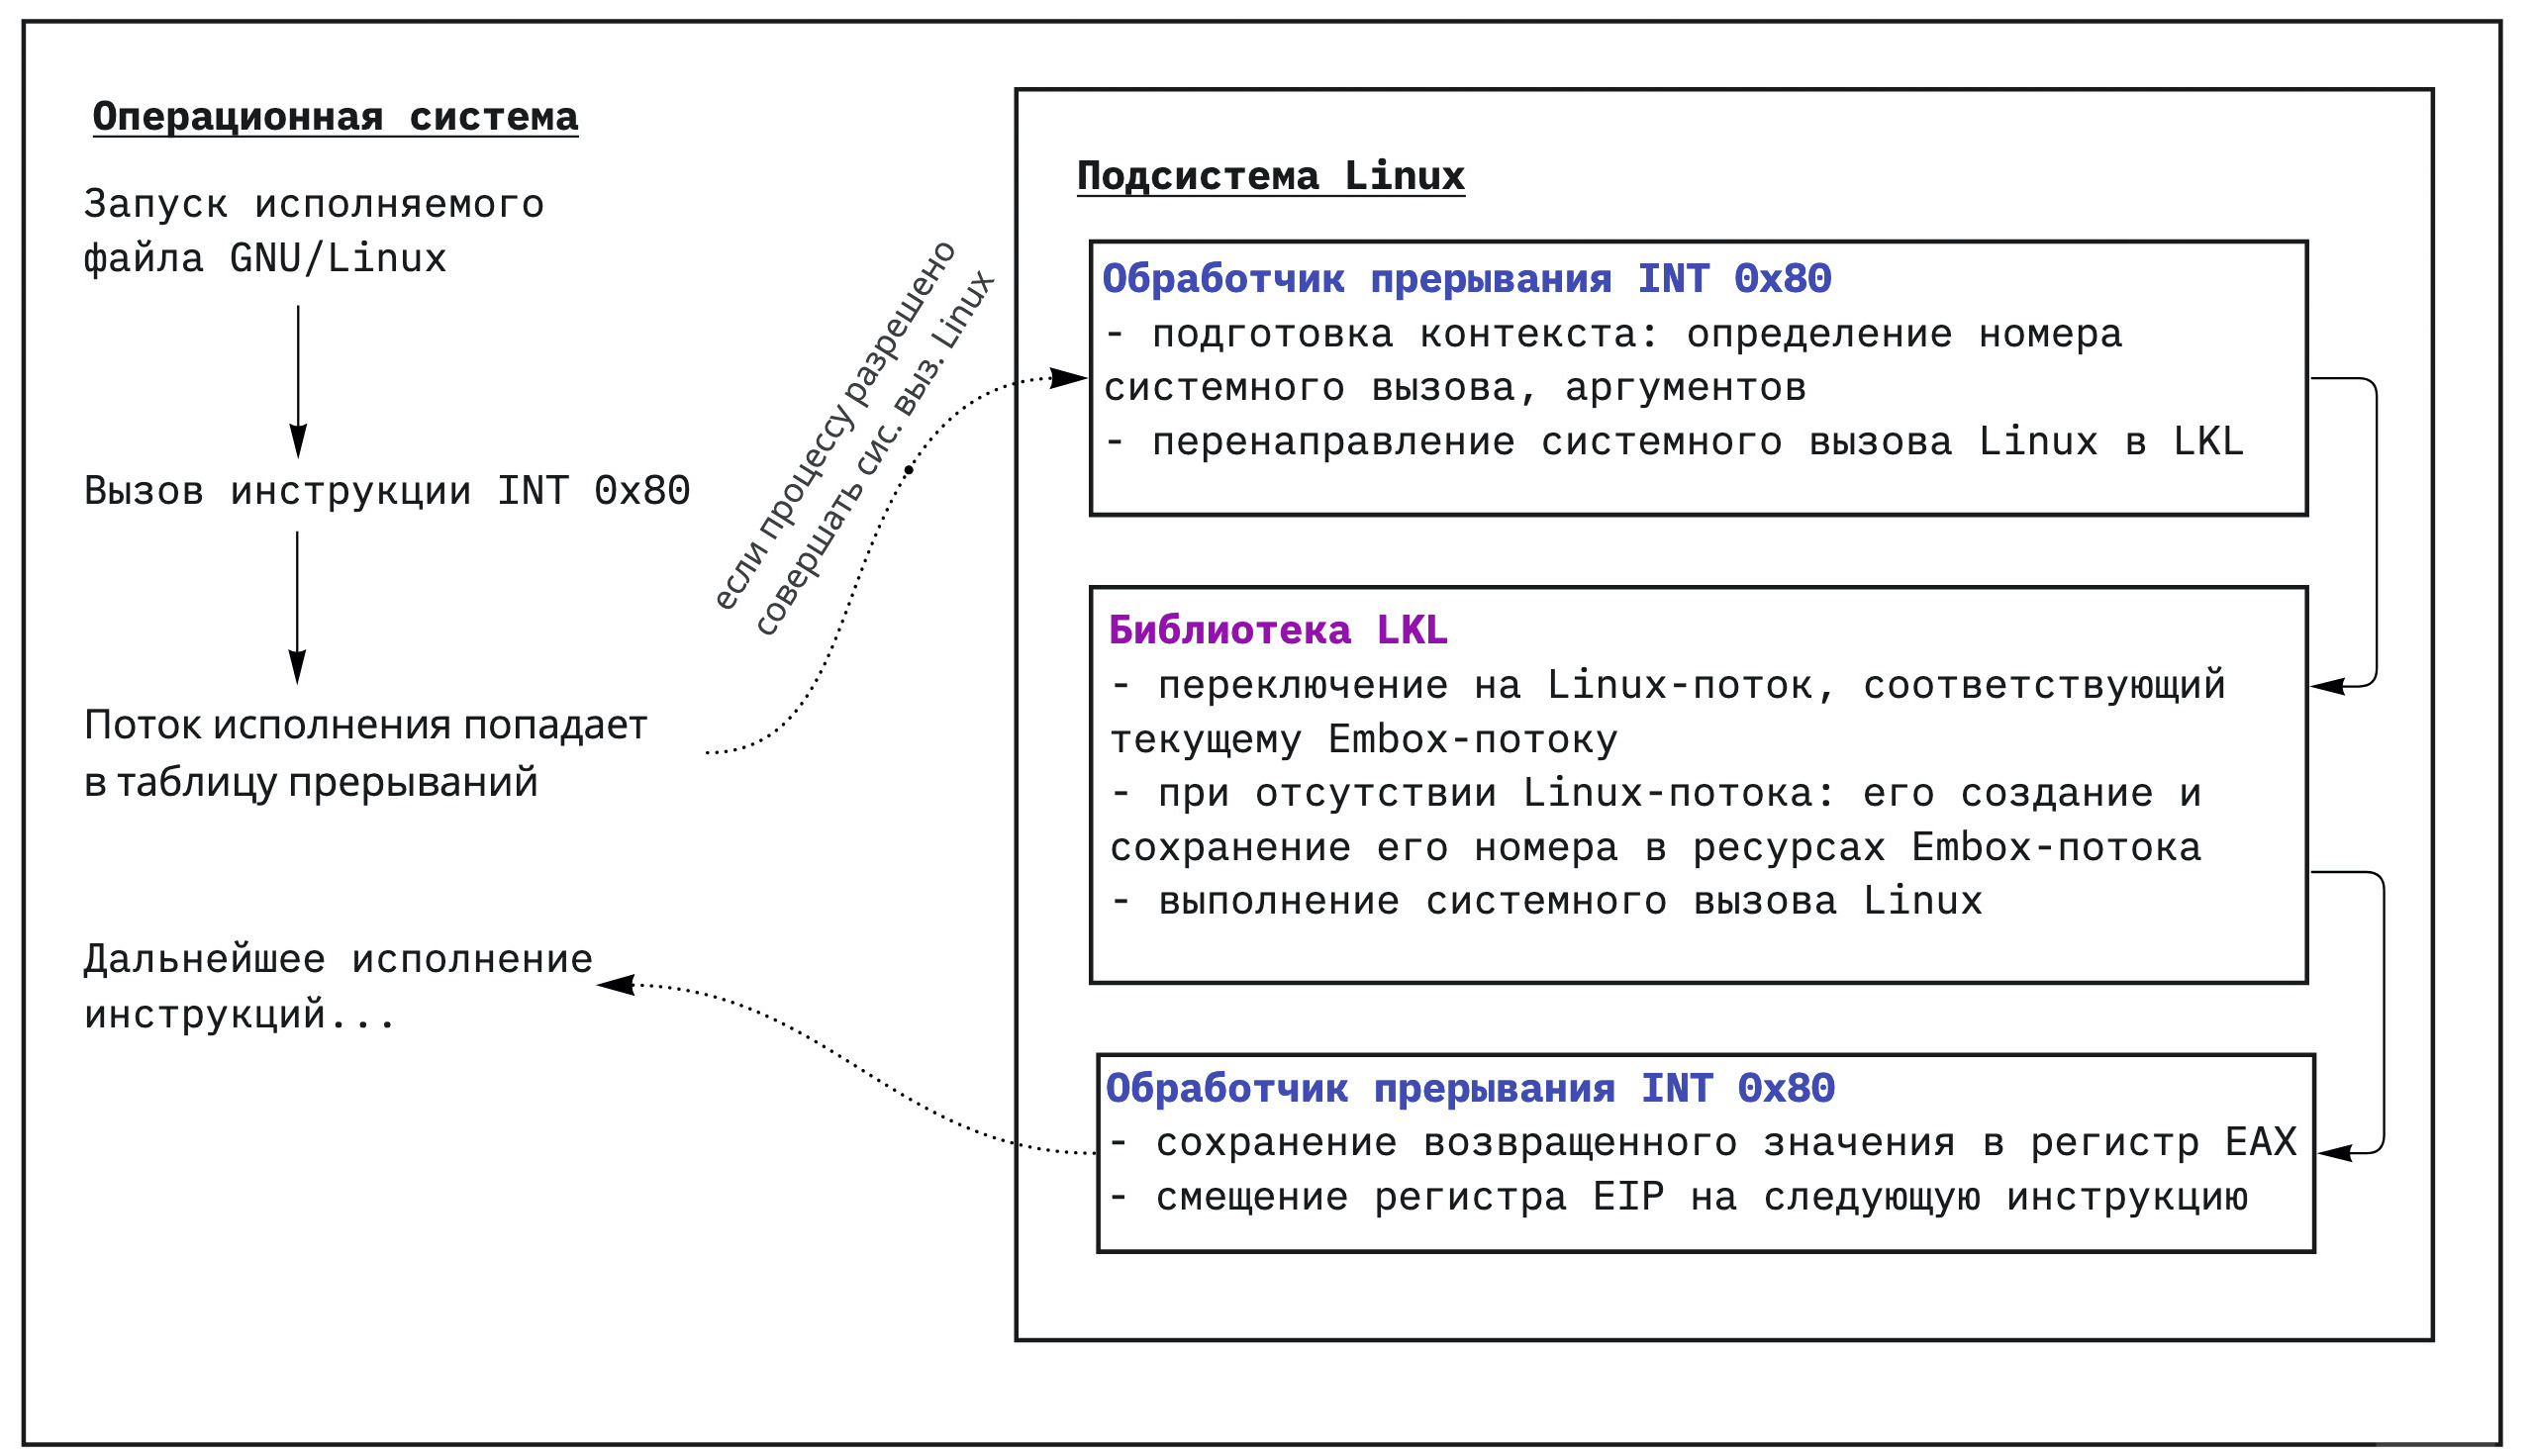
\includegraphics[width=\textwidth]{pictures/Arch.jpg}
\caption{Архитектура слоя совместимости}
\label{fig:arch}
\end{figure}
